\section{DD}

	\begin{frame}[plain]
		\vfill
		\centering
		\begin{beamercolorbox}[sep=8pt,center,shadow=true,rounded=true]{title}
			\textbf{\usebeamerfont{title}\insertsectionhead}\par%
			\color{polimiblue}\noindent\rule{10cm}{1pt} \\
		\end{beamercolorbox}
		\vfill
	\end{frame}

	\subsection{Component View}
		\begin{frame}{High-Level View}
			\centering
			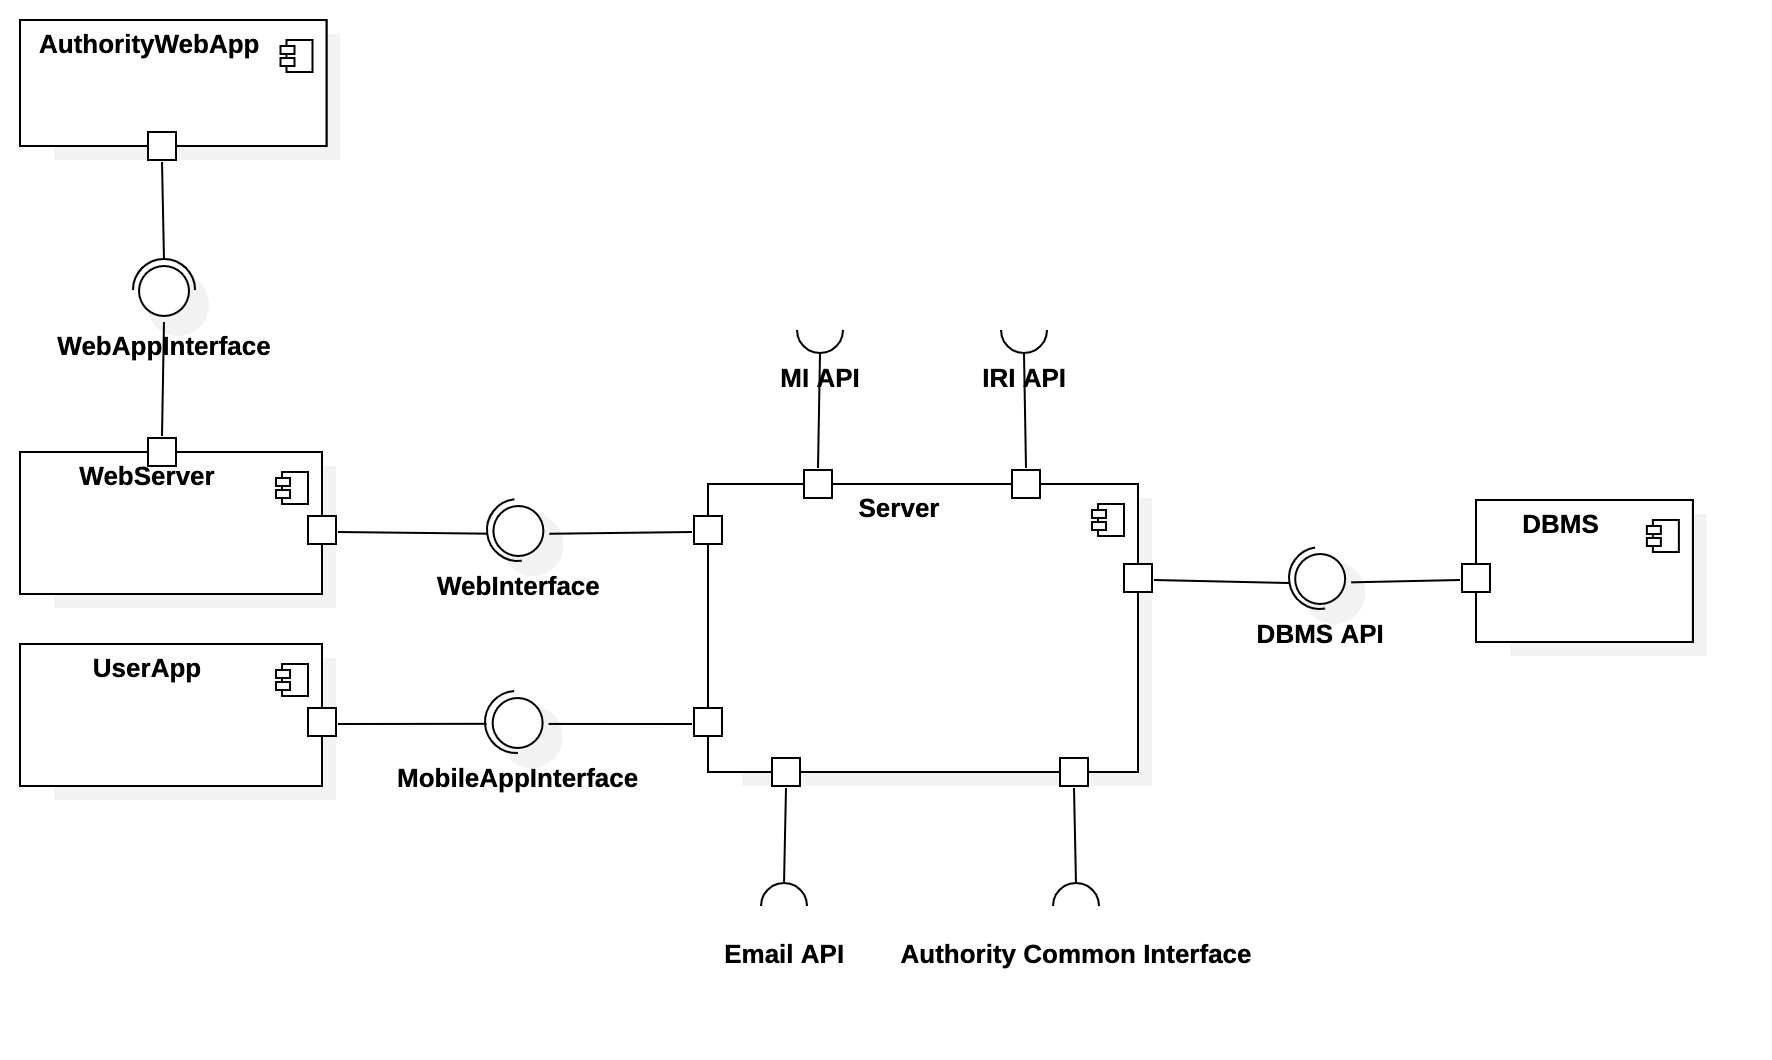
\includegraphics[scale=0.18]{dd/highLevel}
		\end{frame}
	
		\begin{frame}{Server Component}
			\noindent\makebox[\textwidth]{%
			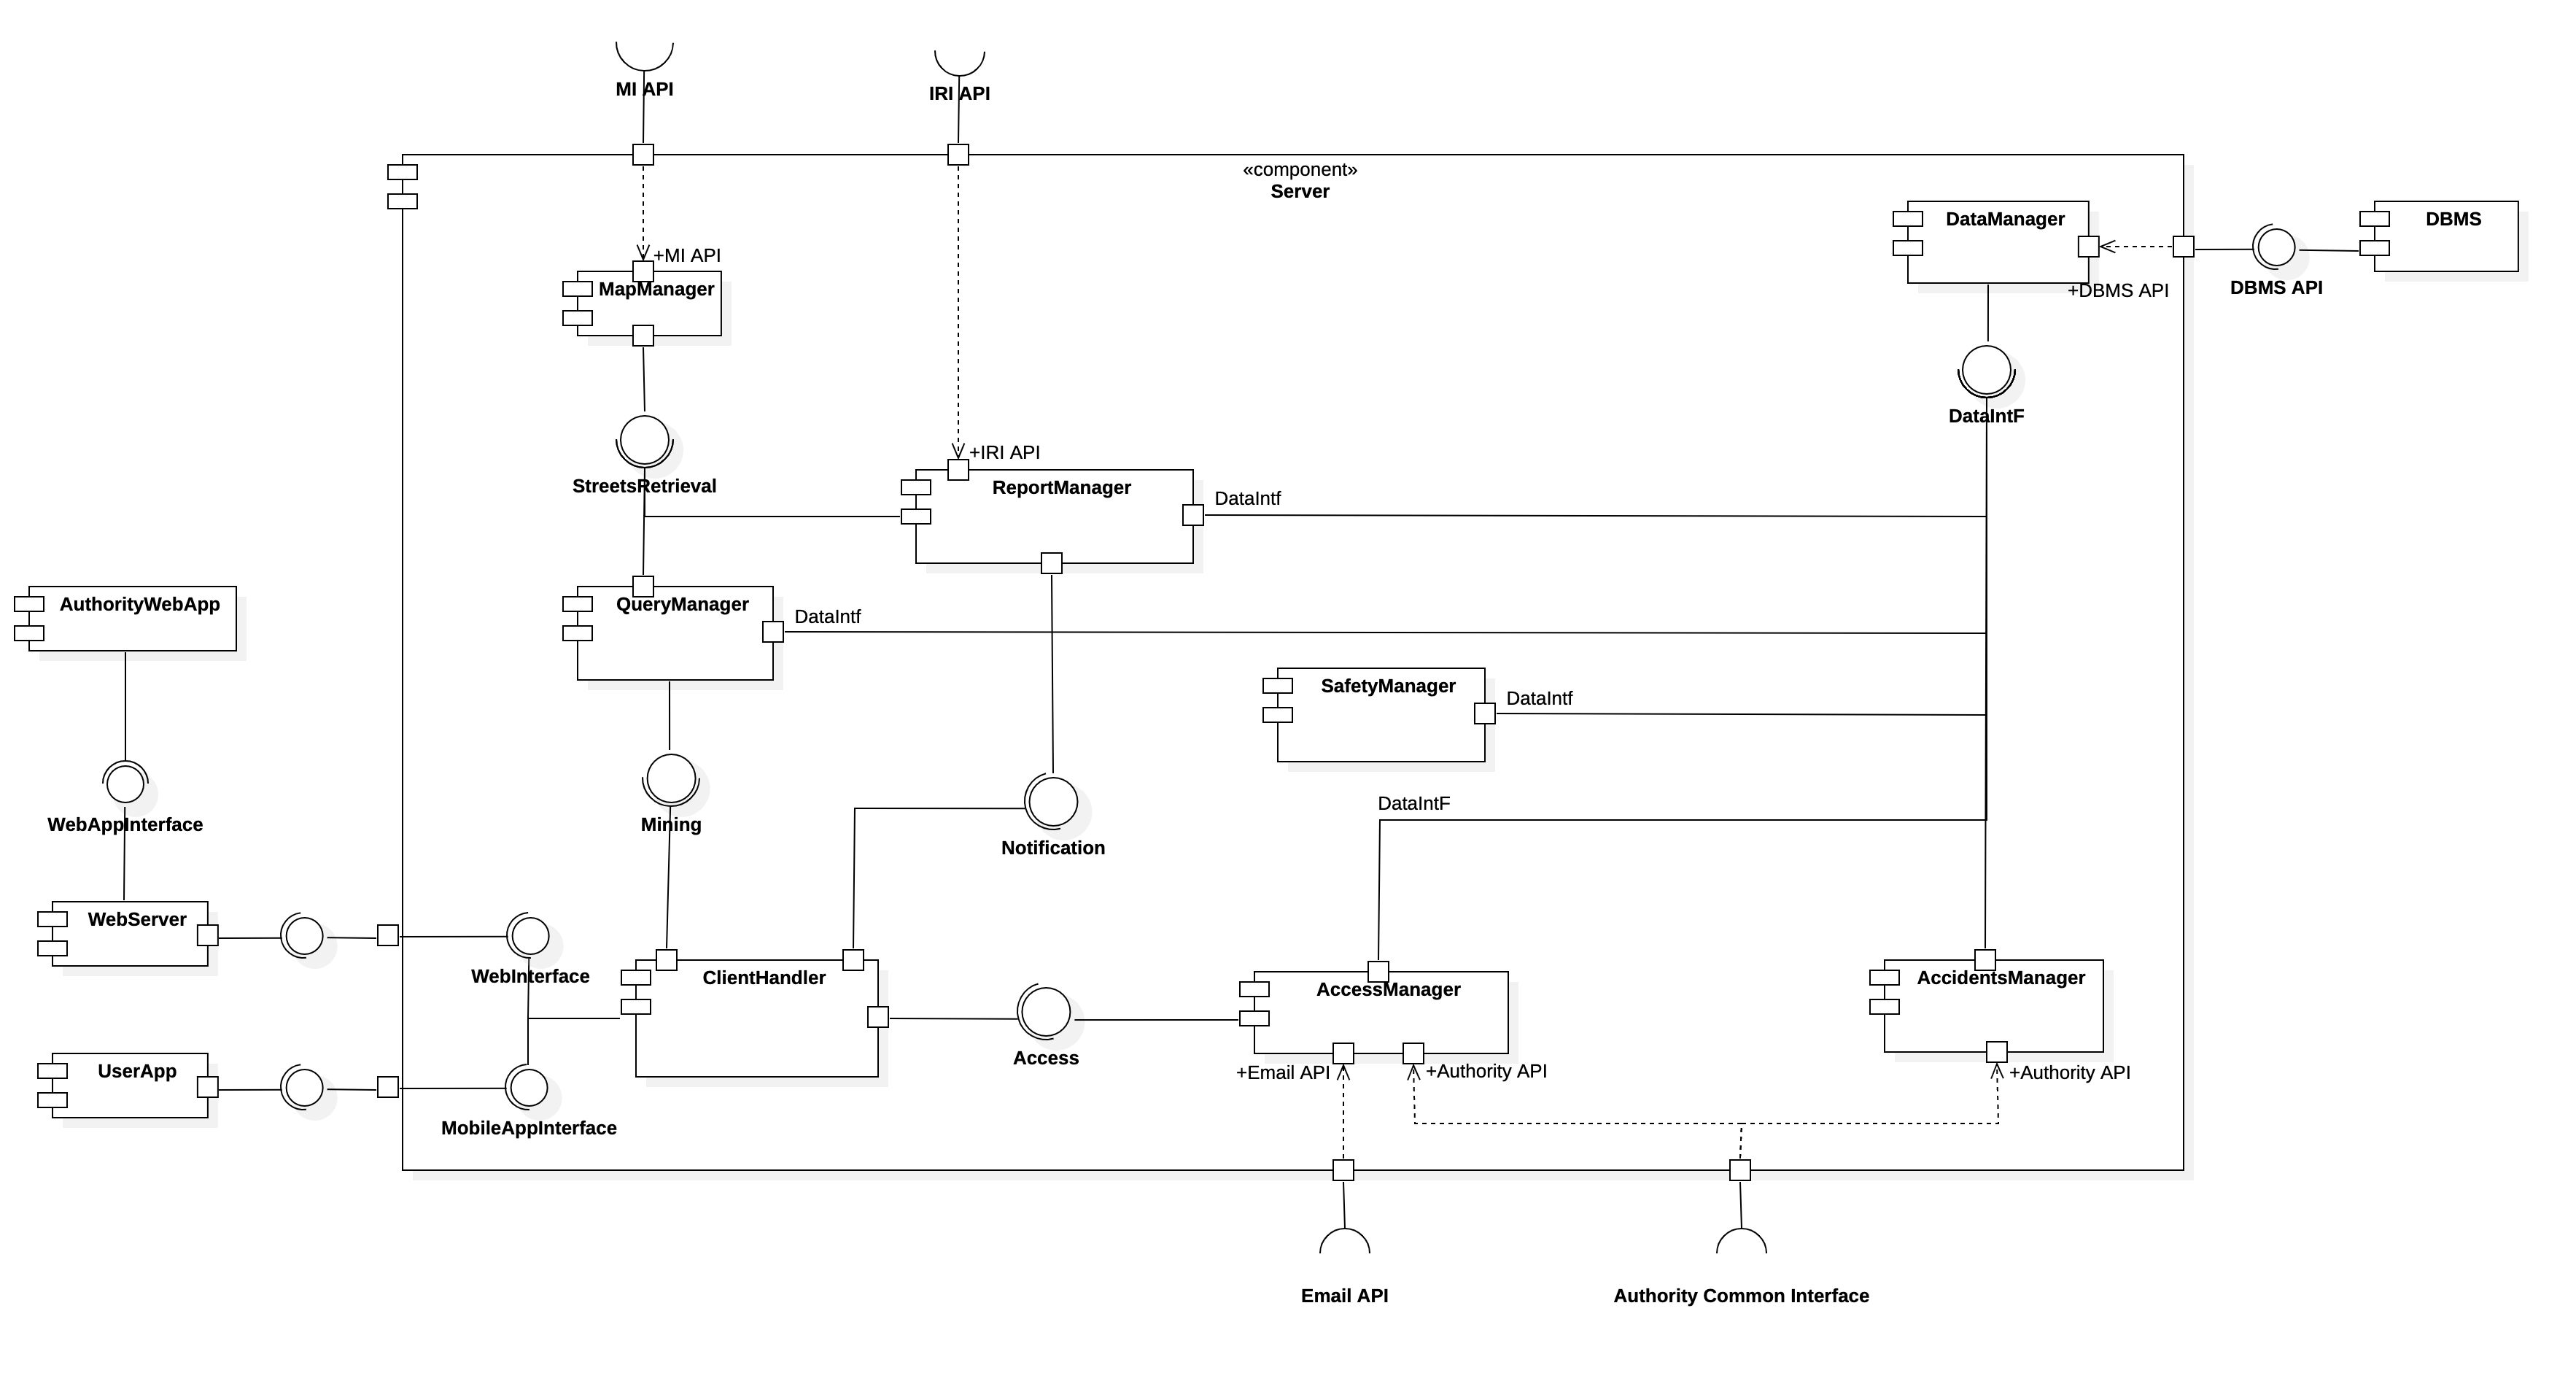
\includegraphics[width=1.2\textwidth]{dd/server}}
		\end{frame}
	
	\subsection{Components Interfaces}
		\begin{frame}{Component Interfaces}
			\vspace{-6pt}
			\noindent\makebox[\textwidth]{%
			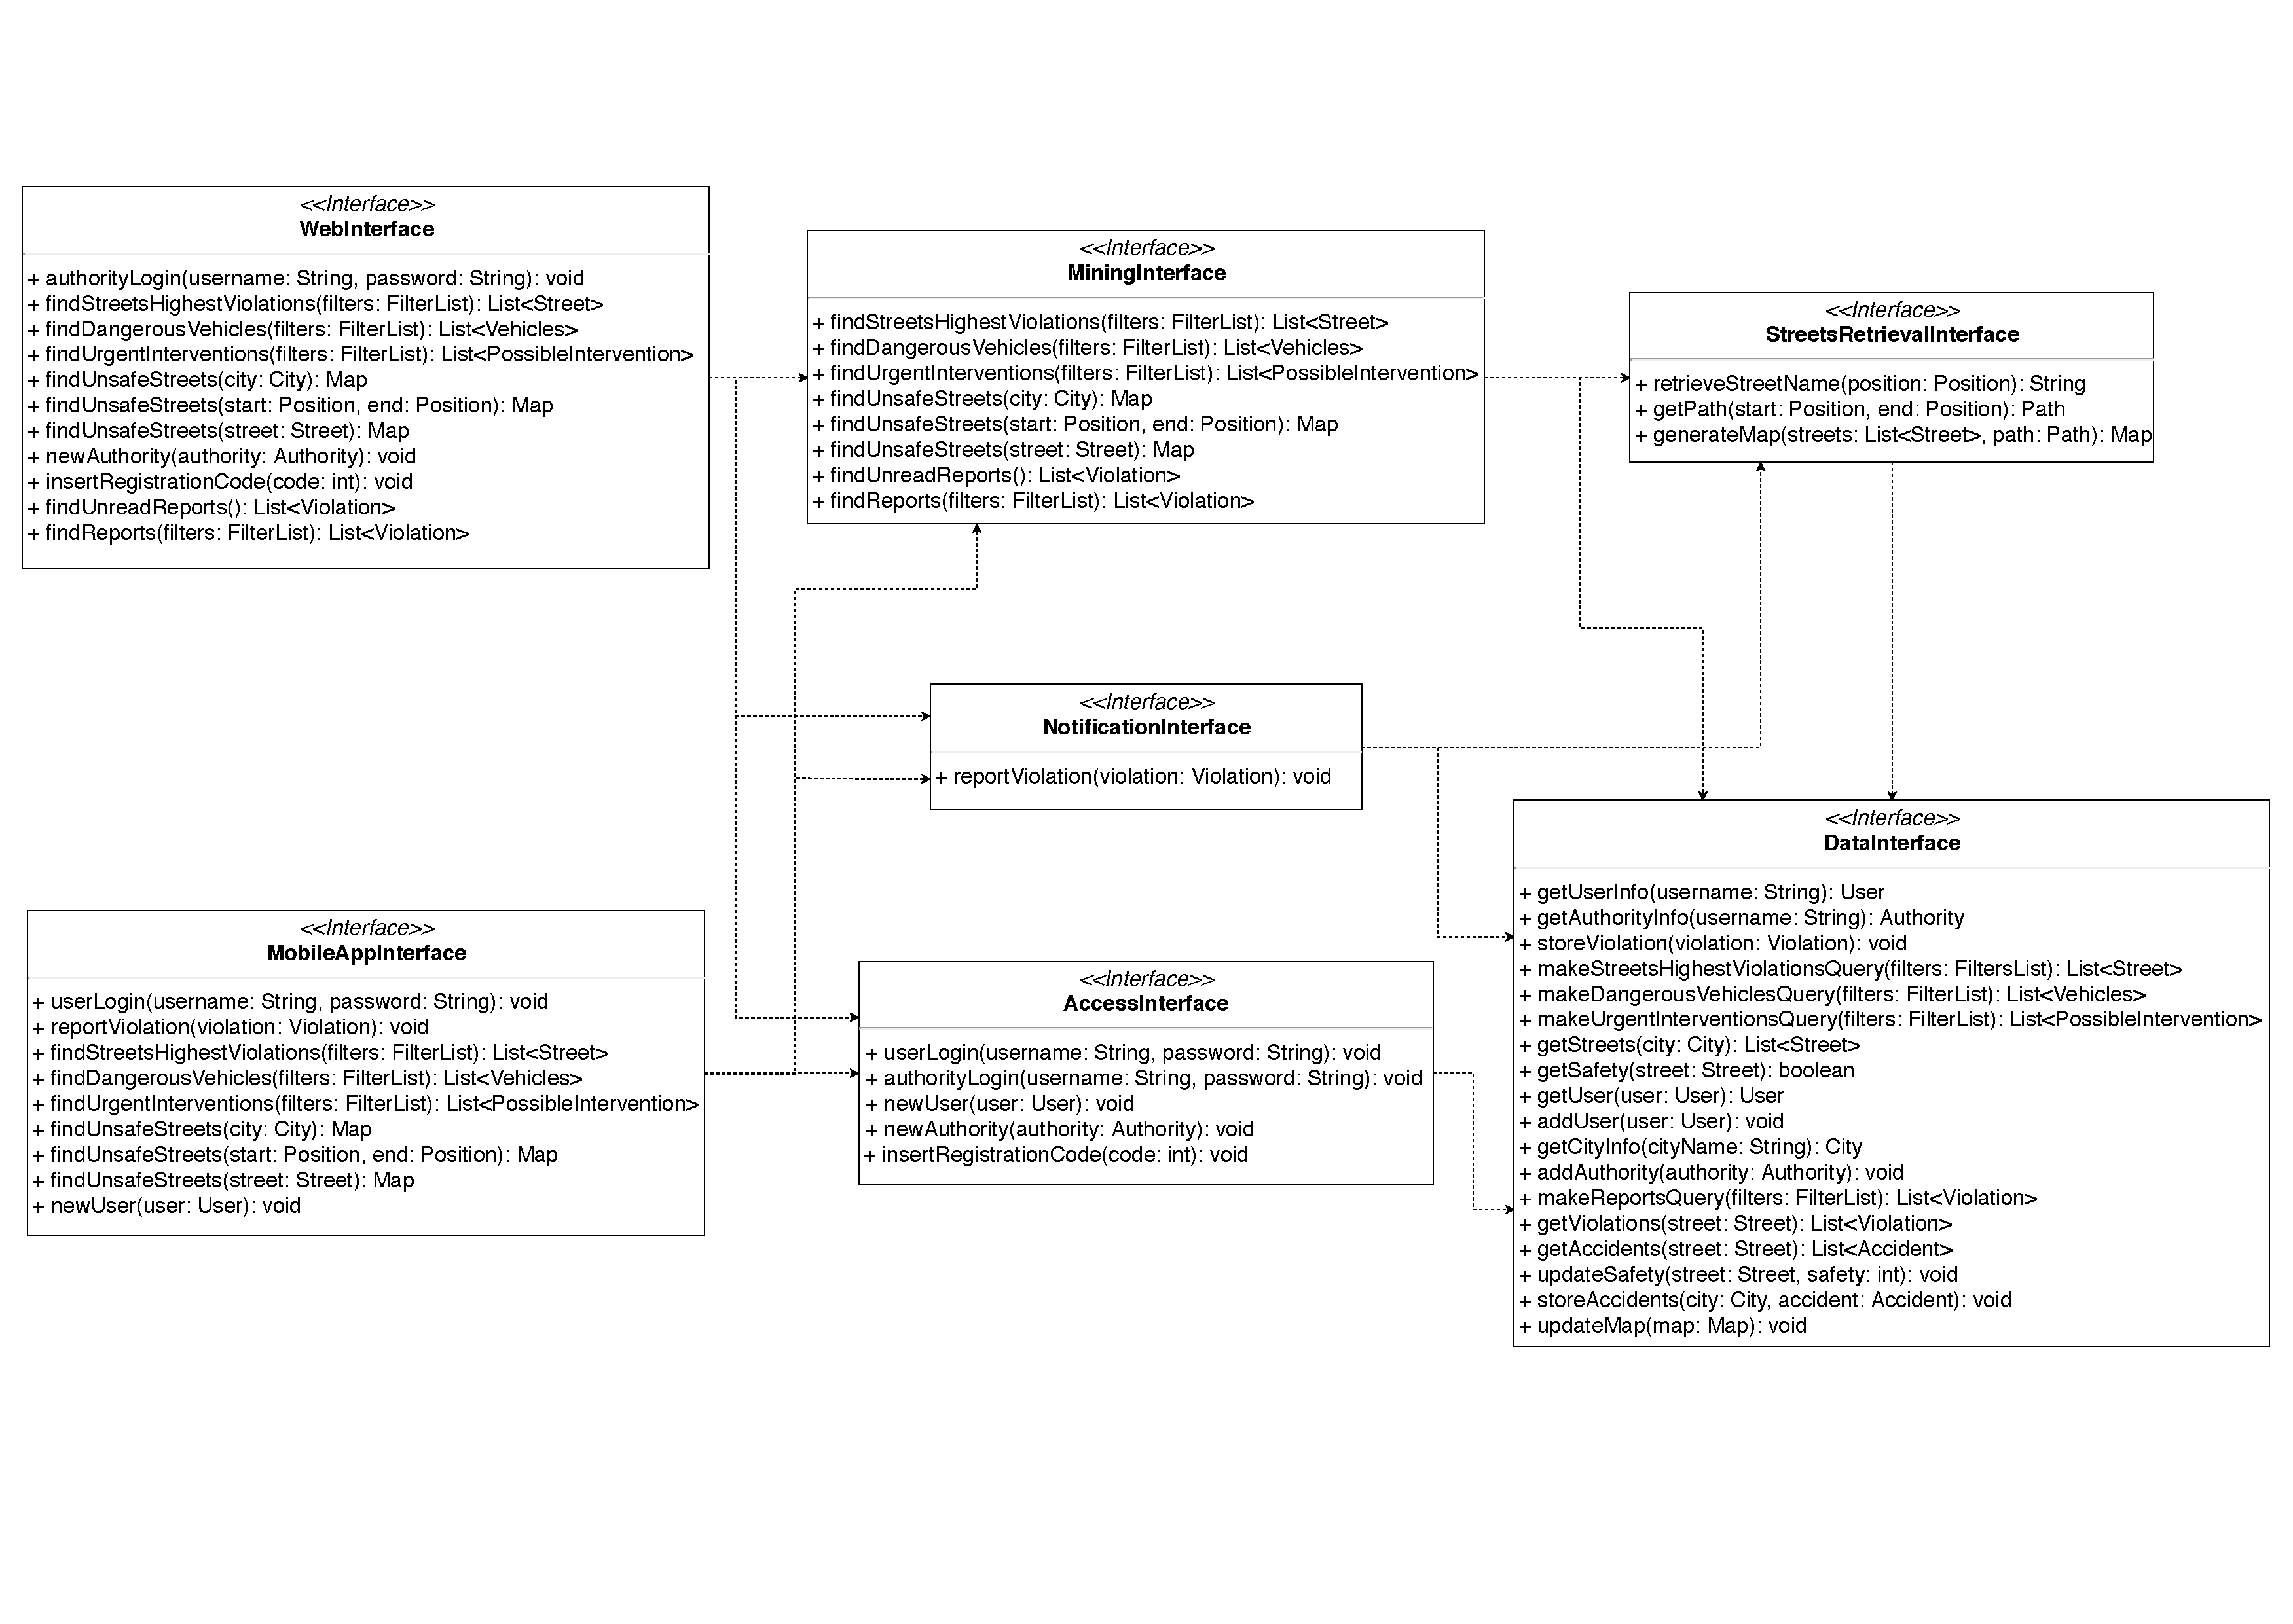
\includegraphics[scale=0.21]{dd/componentInterfaces}}
		\end{frame}
	
	\subsection{Runtime View}
		\begin{frame}{Report Violation and Find Reports}
			\vspace{-5pt}
			\begin{figure}
				\centering
				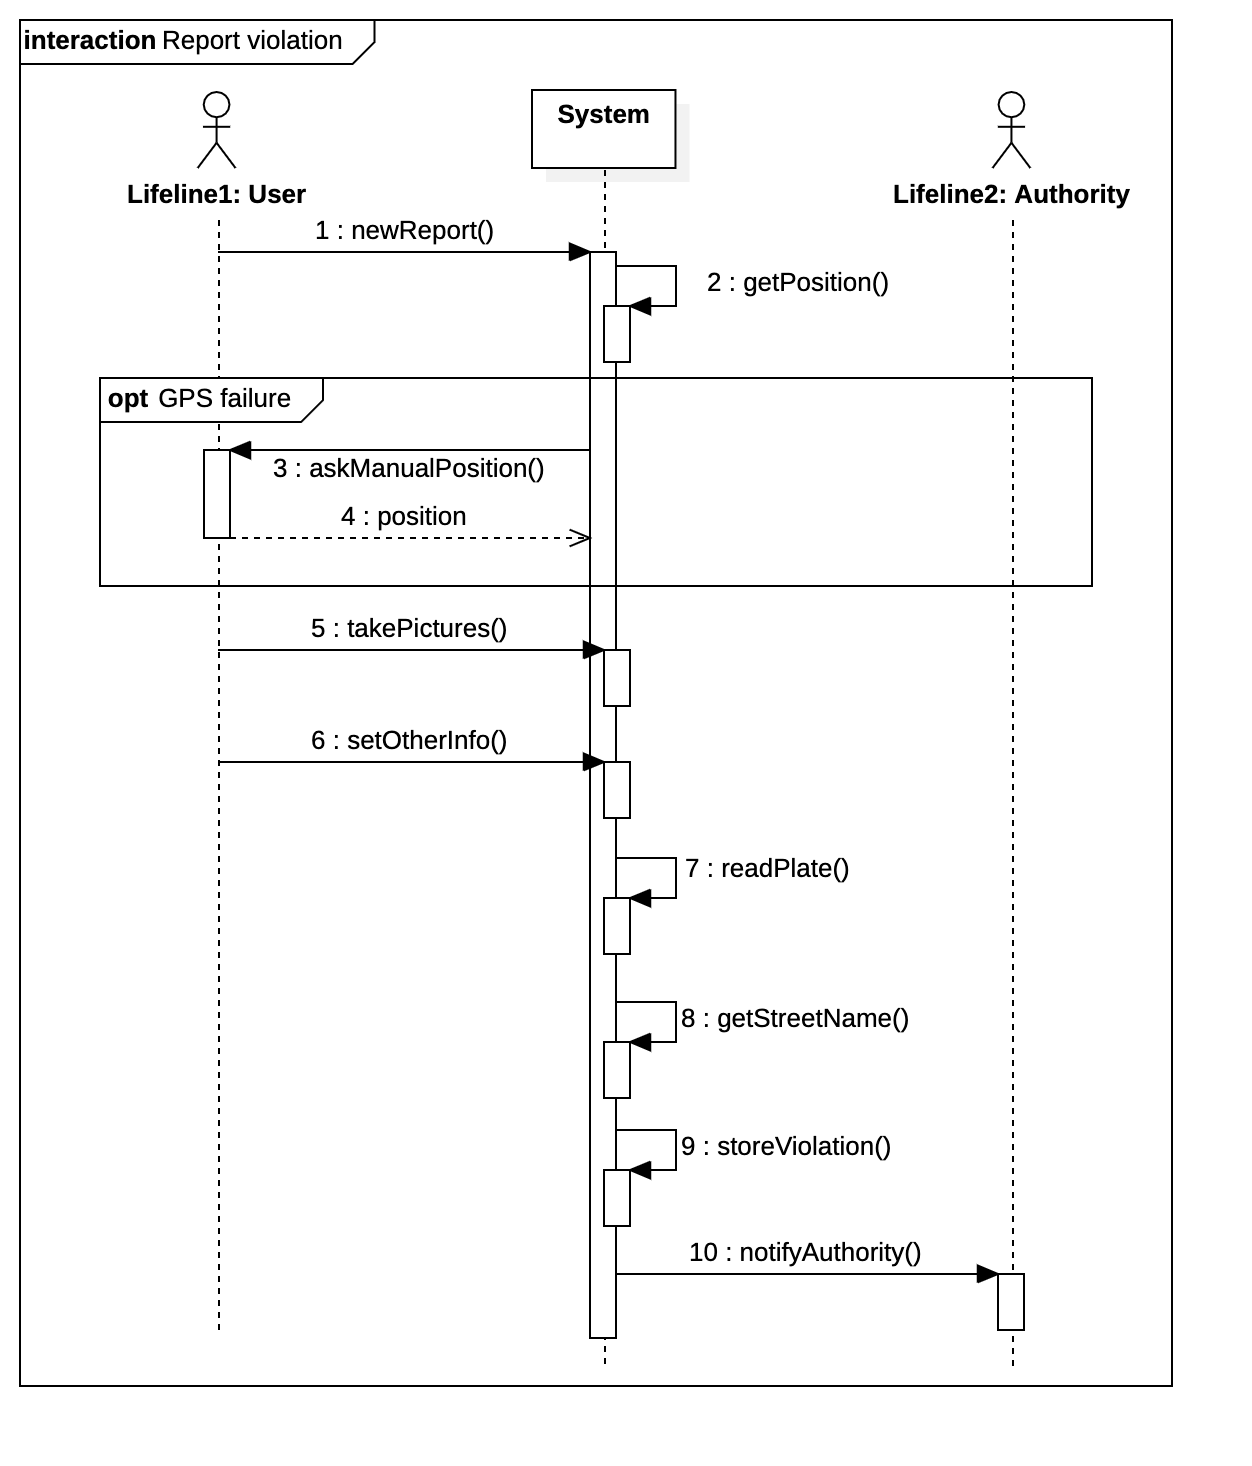
\includegraphics[scale=0.12]{dd/reportViolation}
			\end{figure}
			\vspace{-10pt}
			\begin{figure}
				\centering
				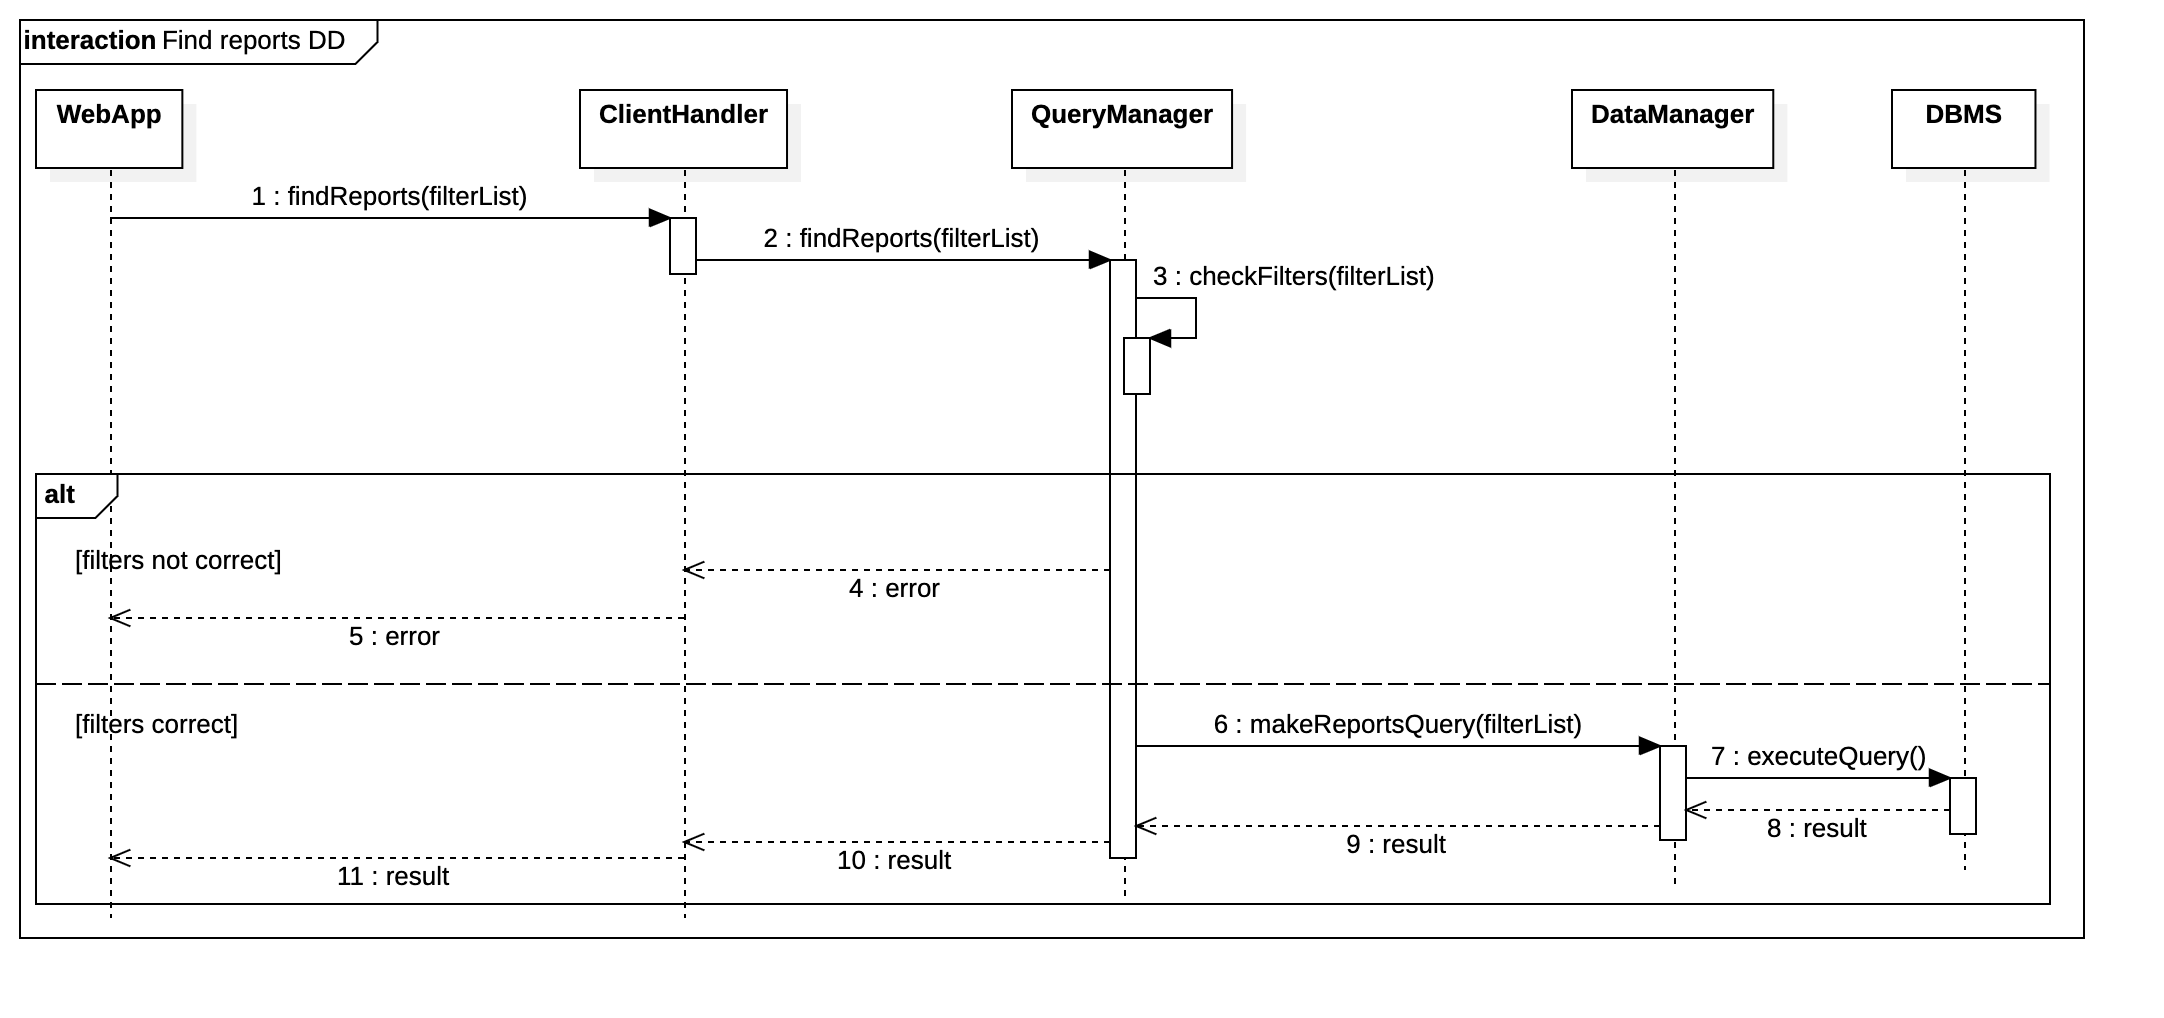
\includegraphics[scale=0.12]{dd/findReports}
			\end{figure}
		\end{frame}
	
		\begin{frame}{Update Safety}
			\begin{figure}[hbtp]
				\centering
				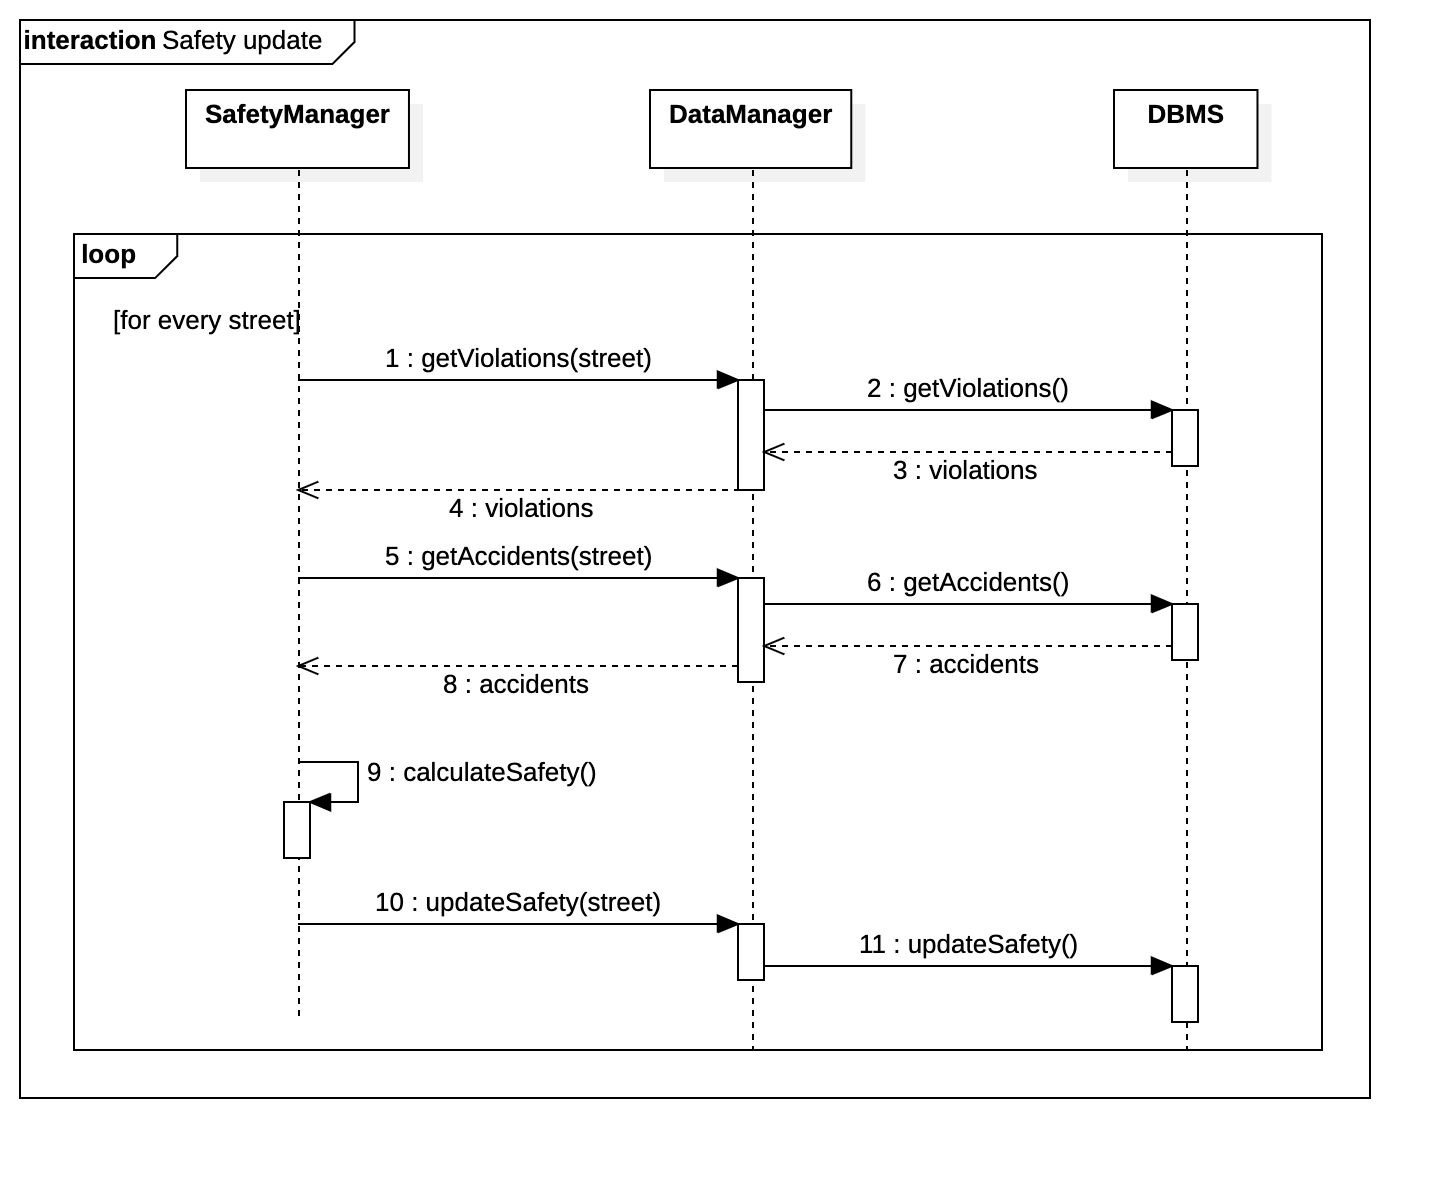
\includegraphics[scale=0.14]{dd/safetyUpdate}
			\end{figure}
		\end{frame}
	
	\subsection{Architectural Styles and Patterns}
		%todo qua dire tutte le cose relative al client-server, 4 tier architecture e REST in modo da collefarsi alla prossima sezione
		\begin{frame}{Client-Server in Four-tier Architecture}
			Architecture
			%todo qua client-server legato a 4tier
		\end{frame}
	
		\begin{frame}{REST and TCP/IP}
			REST
			%todo qua come mai rest e tcp
		\end{frame}
		
	\subsection{Deployment View}
		\begin{frame}{Deployment View}
			\begin{figure}[hbtp]
				\vspace{-10pt}
				\centering
				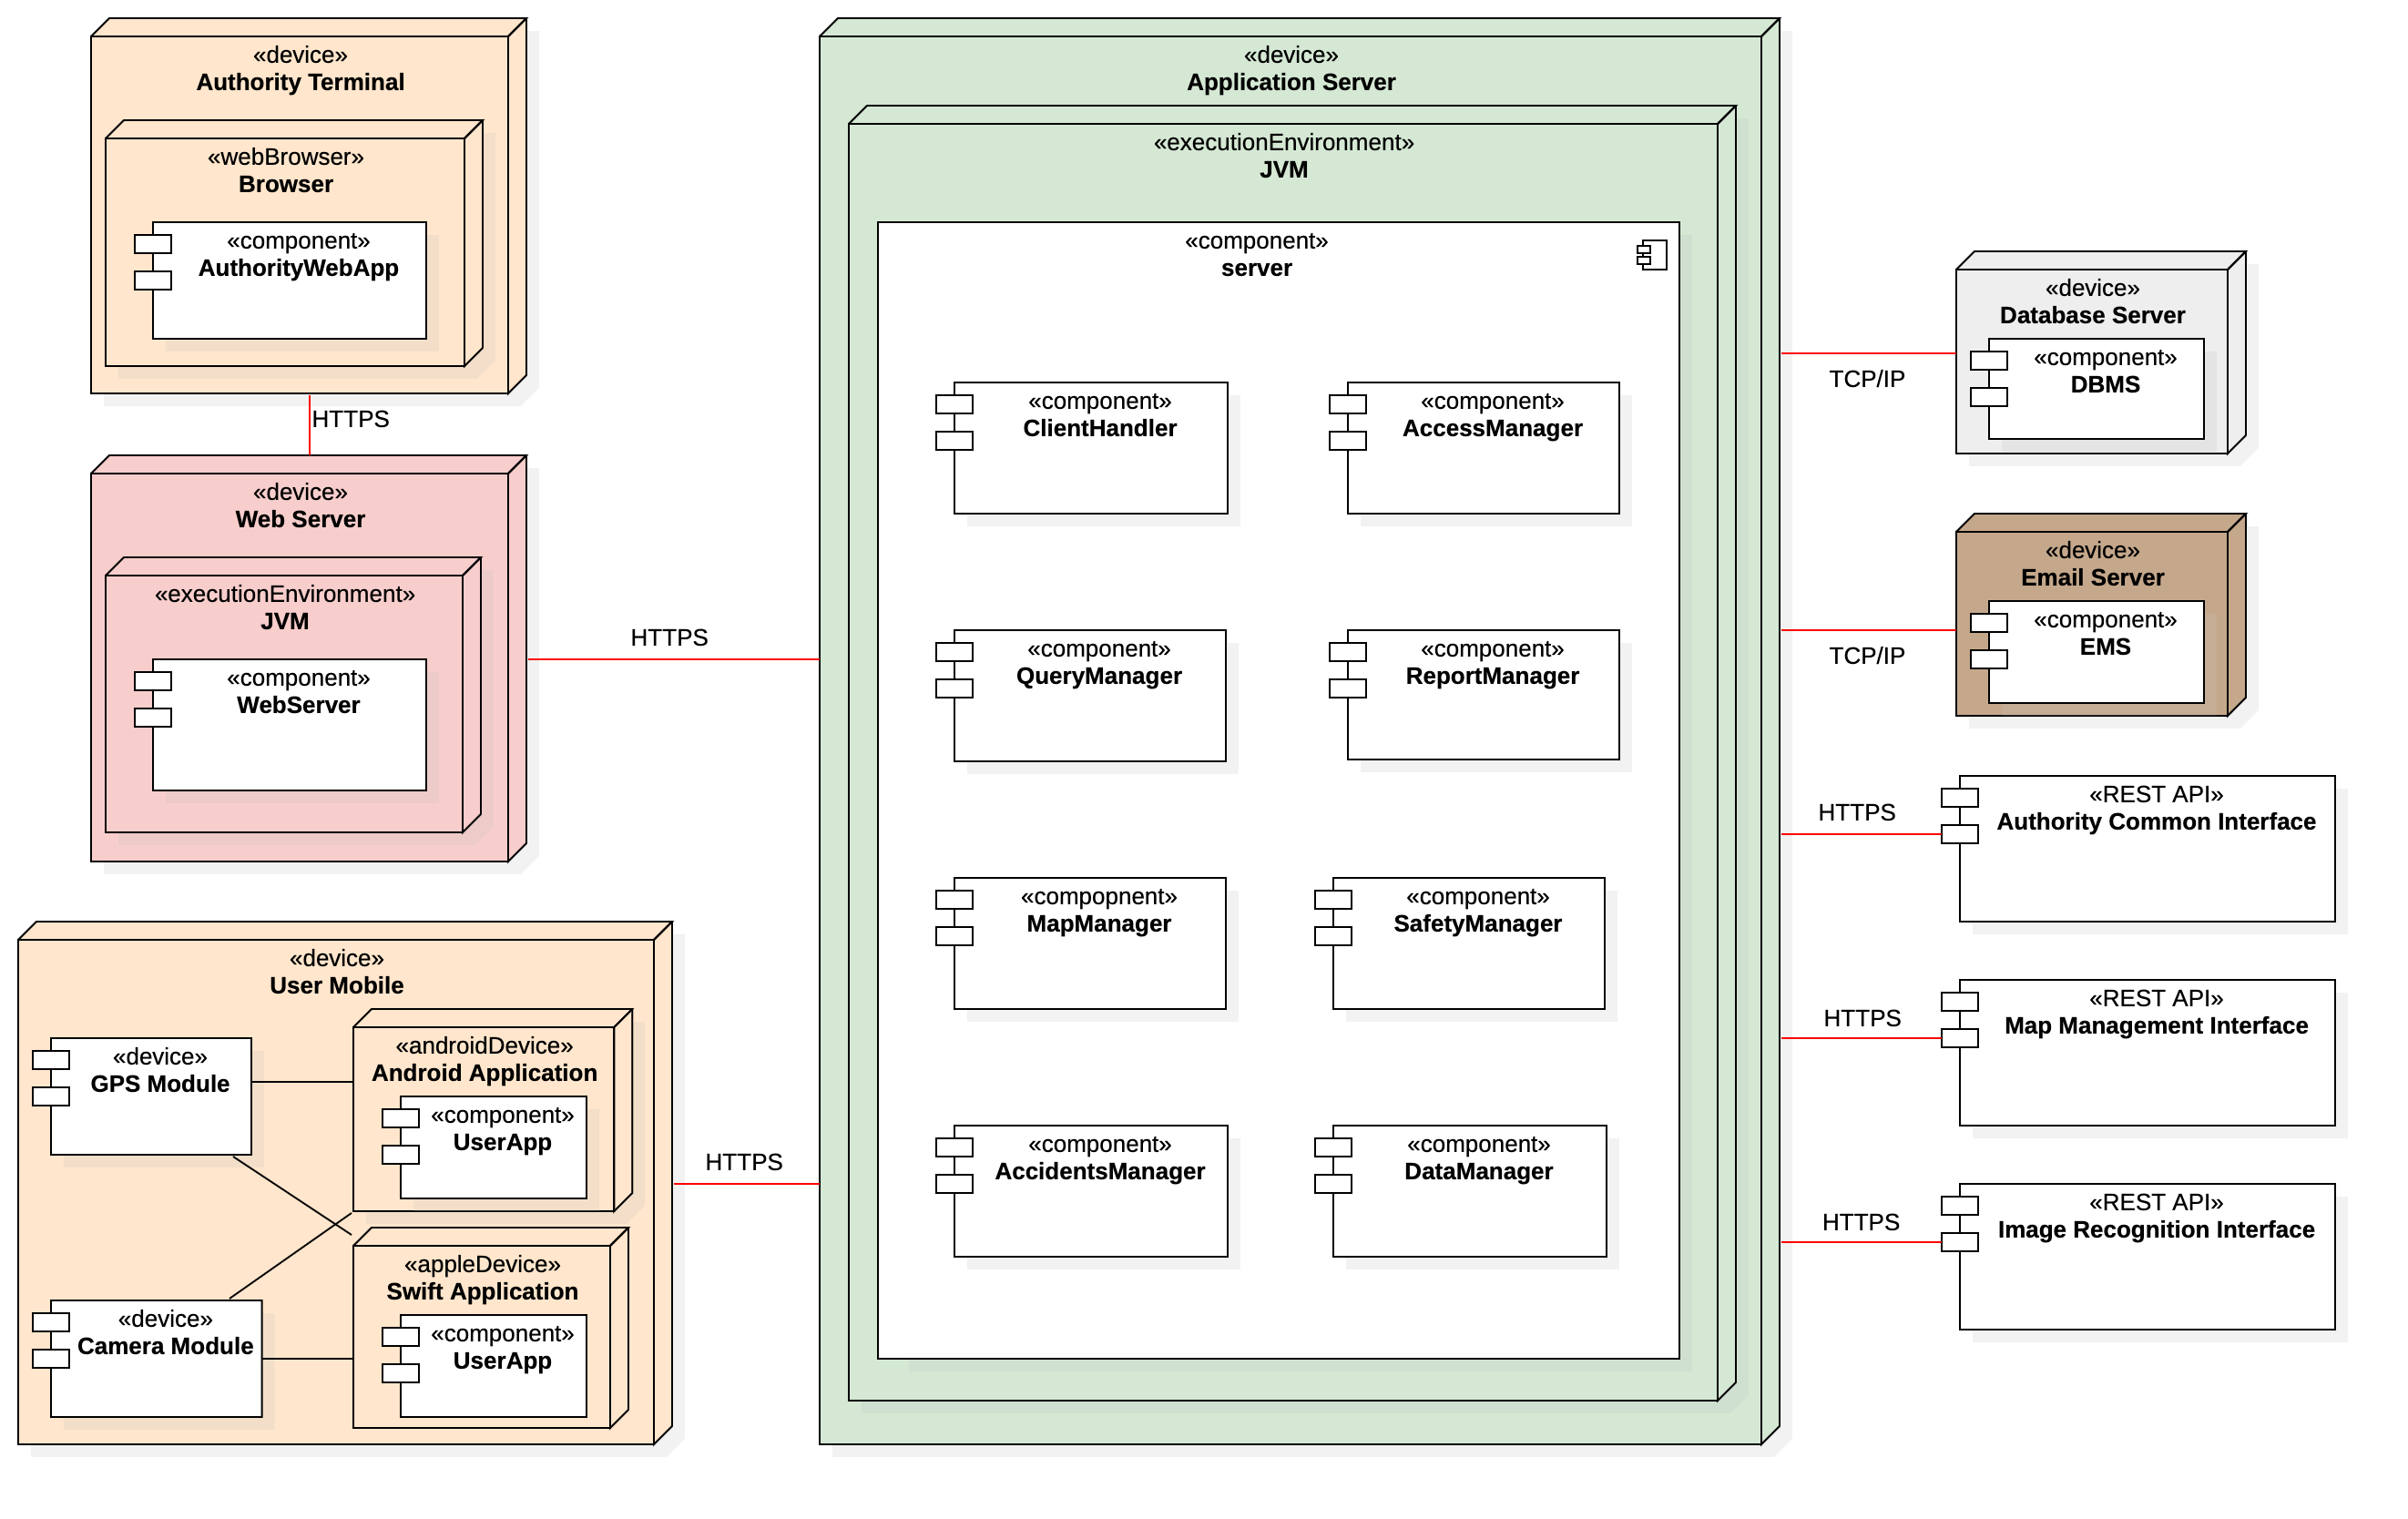
\includegraphics[scale=0.12]{dd/deploymentDiagram}
			\end{figure}
		\end{frame}
	
	\subsection{Implementation Integration and Test Plan}
		\begin{frame}{Strategy Overview}
			\begin{itemize}
				\item First
				\item Second
				\item Third
				\item Fourth
				%todo mettere qua le 4 cose su cui si basa tutto
			\end{itemize}
		\end{frame}
	
		\begin{frame}{Use Relation Hierarchy Diagram}
			\begin{figure}
				\vspace{-10pt}
				\centering
				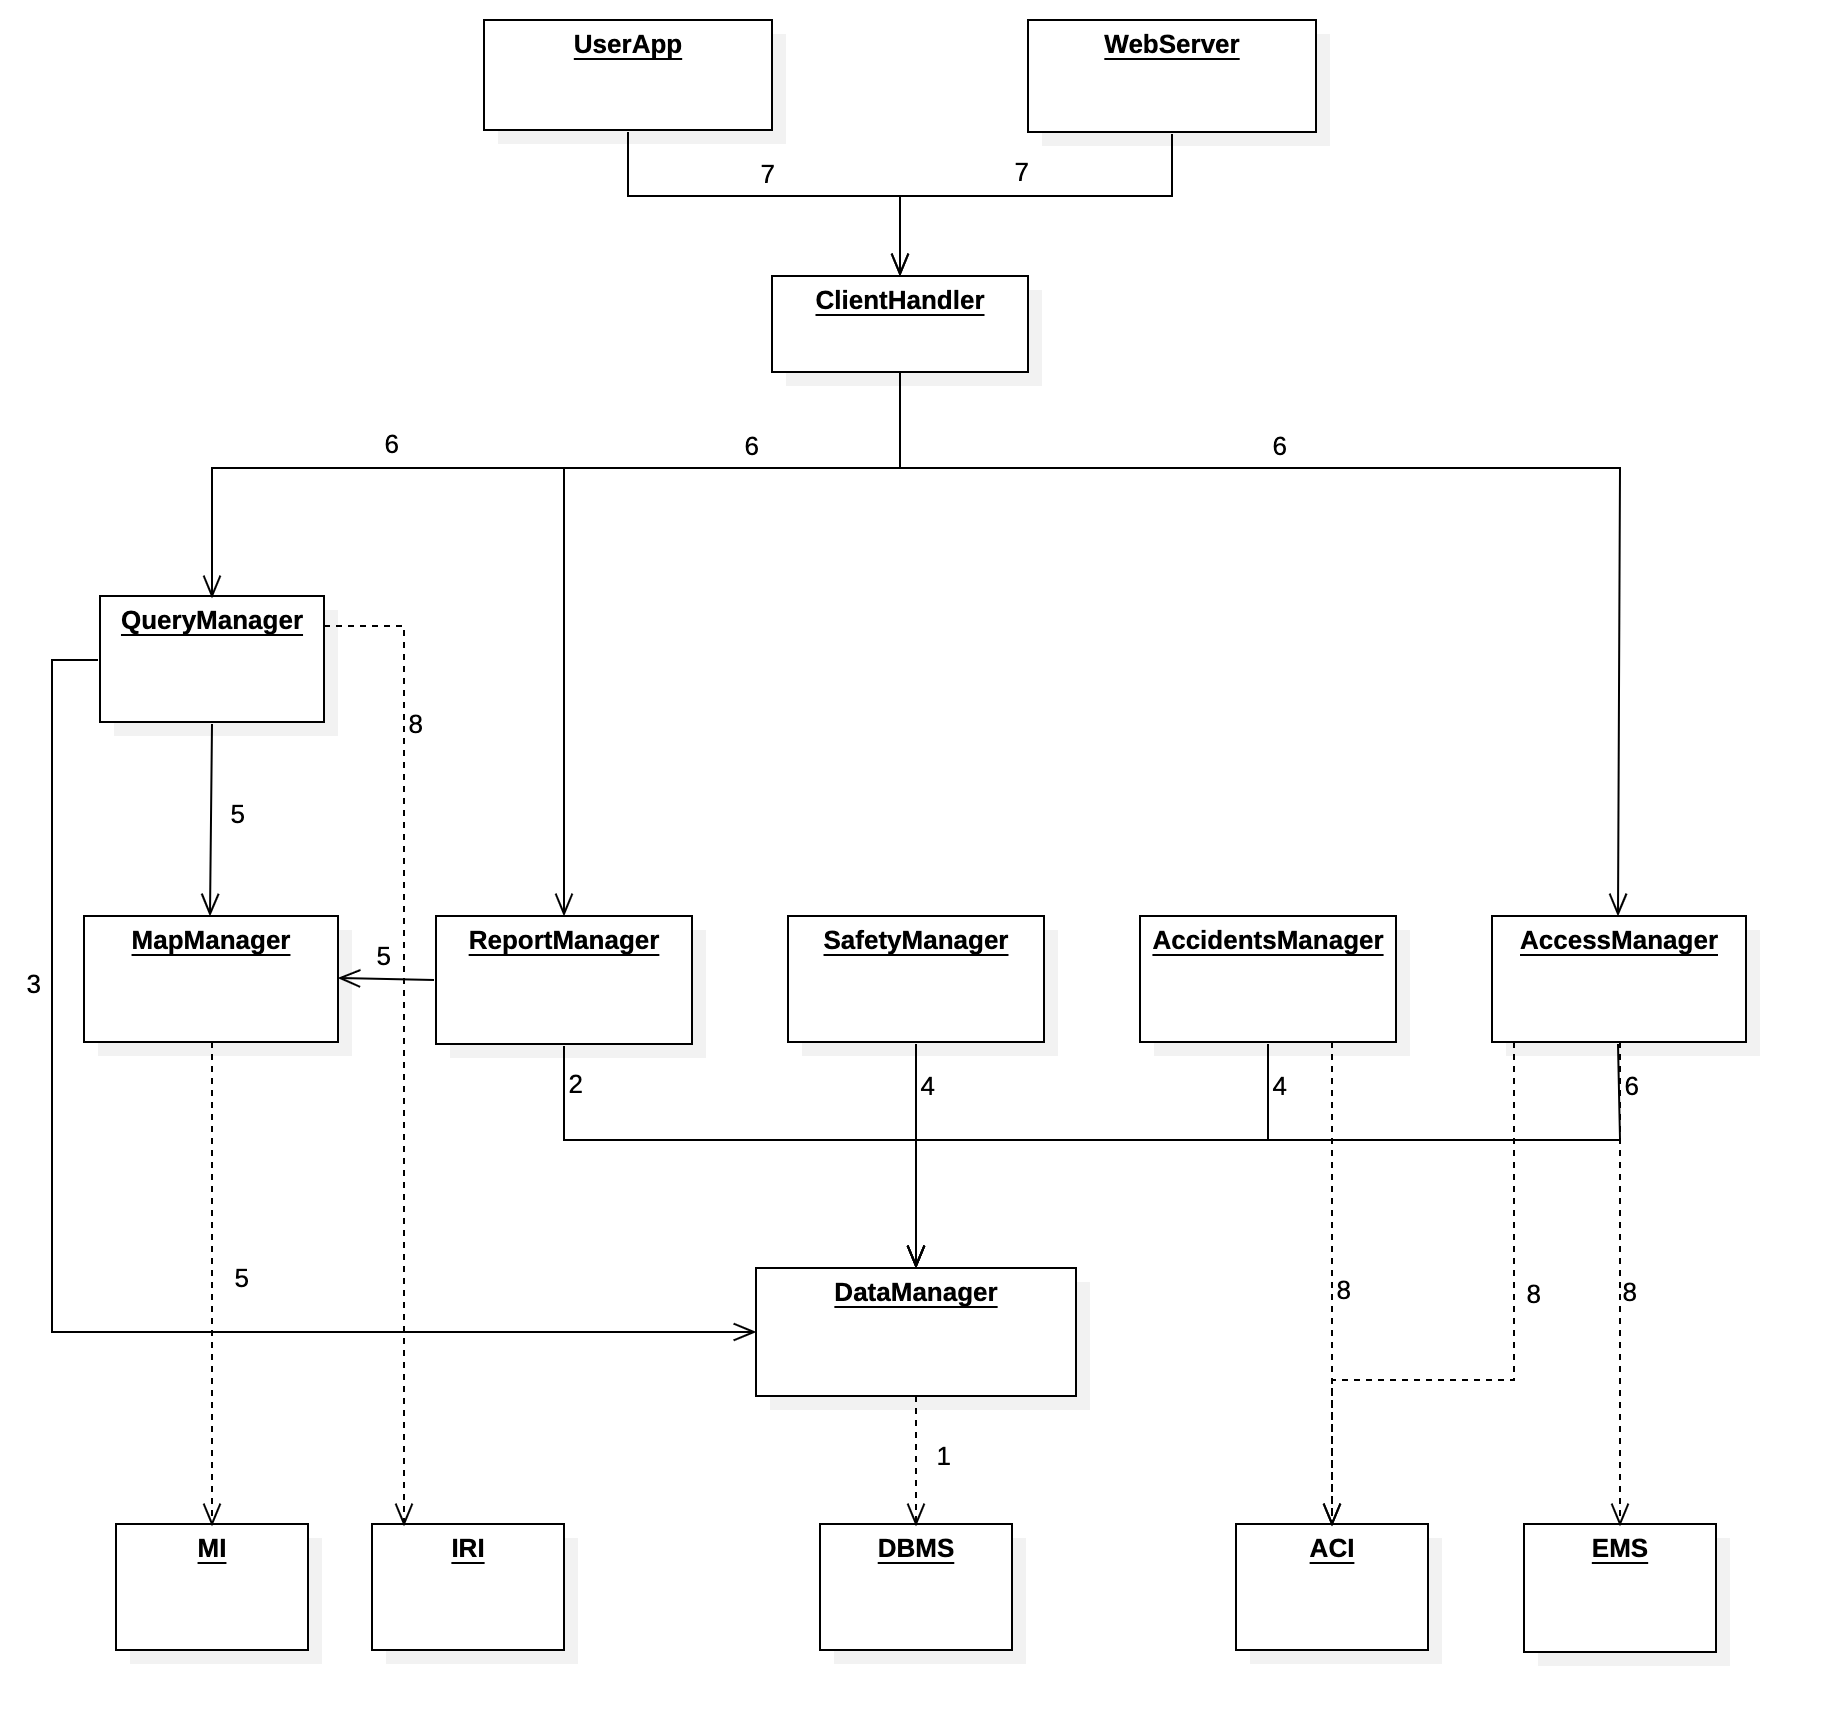
\includegraphics[scale=0.13]{dd/useRelationHierarchy}
			\end{figure}
		\end{frame}